\documentclass[10pt,twocolumn,letterpaper]{article}

\usepackage{cvpr}
\usepackage{times}
\usepackage{epsfig}
\usepackage{graphicx}
\usepackage{amsmath}
\usepackage{amssymb}
\usepackage{tikz}
\usepackage{tikz-qtree}

% Include other packages here, before hyperref.

% If you comment hyperref and then uncomment it, you should delete
% egpaper.aux before re-running latex.  (Or just hit 'q' on the first latex
% run, let it finish, and you should be clear).
\usepackage[breaklinks=true,bookmarks=false]{hyperref}

\cvprfinalcopy % *** Uncomment this line for the final submission

\def\cvprPaperID{****} % *** Enter the CVPR Paper ID here
\def\httilde{\mbox{\tt\raisebox{-.5ex}{\symbol{126}}}}

% Pages are numbered in submission mode, and unnumbered in camera-ready
%\ifcvprfinal\pagestyle{empty}\fi
% \setcounter{page}{4321}
\begin{document}

%%%%%%%%% TITLE
\title{A Survey of NeRF for Sparse Views}

\author{Yuxuan Kuang\\
School of EECS, Peking University\\
% Institution1 address\\
{\tt\small kuangyuxuan@stu.pku.edu.cn}
% For a paper whose authors are all at the same institution,
% omit the following lines up until the closing ``}''.
% Additional authors and addresses can be added with ``\and'',
% just like the second author.
% To save space, use either the email address or home page, not both
% \and
% Second Author\\
% Institution2\\
% First line of institution2 address\\
% {\tt\small secondauthor@i2.org}
}

\maketitle
%\thispagestyle{empty}

%%%%%%%%% ABSTRACT
% \begin{abstract}
%    In this paper, I systematically survey the NeRF model for sparse views.
%    I first analyze the shortcomings and difficulties of the original NeRF model,
%    then I introduce the variants of NeRF for sparse views, analyze their inner relations and compare their abilities.
%    Finally, I point out my personal opinions on the future development of NeRF for sparse views.
% \end{abstract}

%%%%%%%%% BODY TEXT
% introduction
% related works (contributions)
% Relationship between variants
% my opinions and future plans

\section{Introduction}

Neural radiance fields (NeRF)~\cite{mildenhall2020nerf} encode a scene into a neural representation that enables photo-realistic rendering of novel views. However, a successful reconstruction from RGB images requires a large number of input views taken under static conditions — typically up to a few hundred images for room-size scenes.
Moreover, the speed of NeRF is disastrously slow because of the hundreds of views it needs to process.
As a result, how to use NeRF for 3D reconstruction leveraging very few images is quite important.
In the next sections, I will introduce the variants of NeRF that is able to leverage sparse views — even single view to reconstruct 3D scenes.

\section{Related Works}

To tackle the tricky problem, many methods have been proposed.
In Figure \ref{fig:taxonomy}, these methods are grouped into different perspectives that these methods are based on.
For each perspective, a few works will be mentioned and their contributions will be explained.

\begin{figure}[h]
   \begin{center}
      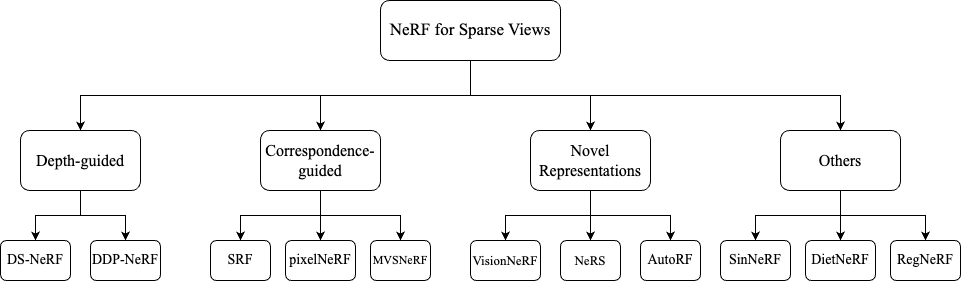
\includegraphics[width=80mm]{assets/taxonomy.png}
   \end{center}
   \caption{Taxonomy of NeRF for Sparse Views}
   \label{fig:taxonomy}
\end{figure}

\subsection{Using Depth to Guide the Reconstruction}

It is very common to use depth information to guide the 3D reconstruction, since the coarse 3D information can be easily obtained from SfM.
In DS-NeRF~\cite{kangle2021dsnerf}, they use SfM to produce sparse 3D points that can be used as “free” depth supervision during training
and add a loss to encourage the distribution of a ray’s terminating depth matches a given 3D keypoint, incorporating depth uncertainty.

While in DDP-NeRF~\cite{Roessle_2022_CVPR}, 

\subsection{Leveraging Correspondences between 2D and 3D}

\subsection{Learning from Psuedo Labels}

\subsection{Others}

\section{Relationship between NeRF Variants}

\section{Future Development}

\newpage
{\small
\bibliographystyle{ieee}
\bibliography{egbib}
}

\end{document}
